\subsection{\Amazon}\label{sec:app_amazon}

In many consumer-facing ML applications, models are trained on data collected on one set of users and then deployed across a wide range of potentially new users. These models can perform well on average but poorly on some individuals \citep{tatman2017,caldas2018leaf,li2019fair,koenecke2020racial}.
These large performance disparities across users are practical concerns in consumer-facing applications, and they can also indicate that models are exploiting biases or spurious correlations in the data \citep{badgeley2019deep,geva2019annotator}.
We study this issue of inter-individual performance disparities on a variant of the \Amazon Reviews dataset \citep{ni2019justifying}.

\subsubsection{Setup}
\paragraph{Problem setting.}
We consider a hybrid domain generalization and subpopulation problem where the domains correspond to different reviewers.
The task is multi-class sentiment classification, where the input $x$ is the text of a review, the label $y$ is a corresponding star rating from 1 to 5, and the domain $d$ is the identifier of the reviewer who wrote the review.
Our goal is to perform consistently well across a wide range of reviewers, i.e., to achieve high tail performance on different subpopulations of reviewers in addition to high average performance. In addition, we consider disjoint set of reviewers between training and test time.

\paragraph{Data.}
The dataset comprises 539,502 customer reviews on Amazon taken from the Amazon Reviews dataset \citep{ni2019justifying}.
Each input example has a maximum token length of 512.
For each example, the following additional metadata is also available at both training and evaluation time: reviewer ID, product ID, product category, review time, and summary.

To reliably measure model performance on each reviewer, we include at least 75 reviews per reviewer in each split.
Concretely, we consider the following splits, where reviewers are randomly assigned to either in-distribution or out-of-distribution sets:
\begin{enumerate}
  \item \textbf{Training:} 245,502 reviews from 1,252 reviewers.
  \item \textbf{Validation (OOD):} 100,050 reviews from another set of 1,334 reviewers, distinct from training and test (OOD).
  \item \textbf{Test (OOD):} 100,050 reviews from another set of 1,334 reviewers, distinct from training and validation (OOD).
  \item \textbf{Validation (ID):} 46,950 reviews from 626 of the 1,252 reviewers in the training set.
  \item \textbf{Test (ID):} 46,950 reviews from 626 of the 1,252 reviewers in the training set.
\end{enumerate}
The reviewers in the train and in-distribution splits; the validation (OOD) split; and the test (OOD) split are all disjoint,
which allows us to test generalization to unseen reviewers.
See \refapp{app_amazon_details} for more details.

\paragraph{Evaluation.}
To assess whether models perform consistently well across reviewers, we evaluate models by their accuracy on the reviewer at the 10th percentile.
This follows the federated learning literature, where it is standard to  measure model performance on devices and users at various percentiles in an effort to encourage good performance across many devices \citep{caldas2018leaf,li2019fair}.

\paragraph{Potential leverage.}
We include more than a thousand reviewers in the training set, capturing variation across a wide range of reviewers.
In addition, we provide reviewer ID annotations for all reviews in the dataset.
These annotations could be used to directly mitigate performance disparities across reviewers seen during training time.

\subsubsection{Baseline results}
\begin{table*}[tbp]
  \caption{Baseline results on \Amazon. We report the accuracy of models trained using ERM, CORAL, IRM, and group DRO, as well as a reweighting baseline that reweights for class balance. To measure tail performance across reviewers, we report the accuracy for the reviewer in the 10th percentile. While the performance drop on \Amazon is primarily from subpopulation shift, there is also a performance drop from evaluating on unseen reviewers, as evident in the gaps in accuracies between the in-distribution and the out-of-distribution sets.
  }\label{tab:results_amazon}
  \centering
  \begin{adjustbox}{width=1\textwidth}
  \begin{tabular}{lcccccccc}
  \toprule
    & \multicolumn{2}{c}{Validation (ID)} & \multicolumn{2}{c}{Validation (OOD)} & \multicolumn{2}{c}{Test (ID)} & \multicolumn{2}{c}{Test (OOD)}\\
  Algorithm & 10th percentile & Average & 10th percentile & Average & 10th percentile & Average & 10th percentile & Average \\
  \midrule
ERM & 58.7 (0.0) & 75.7 (0.2) & 55.2 (0.7) & 72.7 (0.1) & \textbf{57.3} (0.0) & \textbf{74.7} (0.1) & \textbf{53.8} (0.8) & \textbf{71.9} (0.1) \\
CORAL & 56.2 (1.7) & 74.4 (0.3) & 54.7 (0.0) & 72.0 (0.3) & 55.1 (0.4) & 73.4 (0.2) & 52.9 (0.8) & 71.1 (0.3) \\
IRM & 56.4 (0.8) & 74.3 (0.1) & 54.2 (0.8) & 71.5 (0.3) & 54.7 (0.0) & 72.9 (0.2) & 52.4 (0.8) & 70.5 (0.3) \\
Group DRO & 57.8 (0.8) & 73.7 (0.6) & 54.7 (0.0) & 70.7 (0.6) & 55.8 (1.0) & 72.5 (0.3) & 53.3 (0.0) & 70.0 (0.5) \\
Reweighted (label)  & 55.1 (0.8) & 71.9 (0.4) & 52.1 (0.2) & 69.1 (0.5) & 54.4 (0.4) & 70.7 (0.4) & 52.0 (0.0) & 68.6 (0.6)\\
  \bottomrule
  \end{tabular}
  \end{adjustbox}
\end{table*}

\begin{figure}[!tbp]
  \centering
  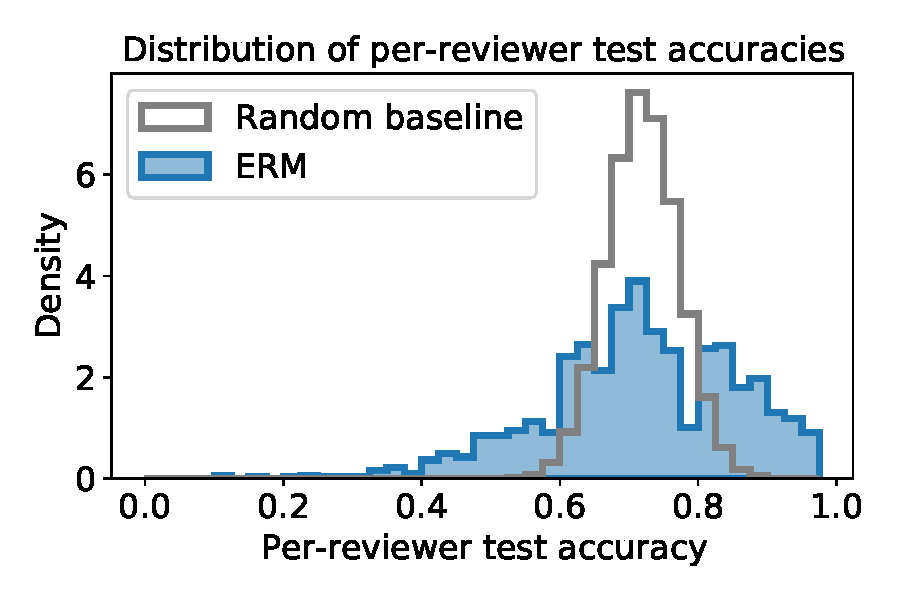
\includegraphics[width=0.5\linewidth]{figures/amazon_acc_histogram.pdf}
  \caption{
    Distribution of per-reviewer accuracy on the test set for the ERM model (blue). The corresponding random baseline would have per-reviewer accuracy distribution in grey.
    }
  \label{fig:result_amazon}
\end{figure}
\paragraph{Model.}
For all experiments, we finetuned DistilBERT-base-uncased models \citep{sanh2019distilbert}, using the implementation from \citet{wolf2019transformers}, and with the following hyperparameter settings:
batch size 8; learning rate $1 \times 10^{-5}$ with the AdamW optimizer \citep{loshchilov2019decoupled}; $L_2$-regularization strength $0.01$; 3 epochs with early stopping; and a maximum number of tokens of 512.
We selected the above hyperparameters based on a grid search over learning rates $\{1 \times 10^{-6}, 2 \times 10^{-6}, 1 \times 10^{-5}, 2 \times 10^{-5}\}$, and all other hyperparameters were simply set to standard/default values.


\paragraph{ERM results and performance drops.}
A DistilBERT-base-uncased model trained with the standard ERM objective performs well on average, but performance varies widely across reviewers (\reffig{result_amazon}, \reftab{results_amazon}).
Despite the high average accuracy of 71.9\%, per-reviewer accuracies vary widely between 100.0\% and 12.0\%, with accuracy at the 10th percentile of 53.8\%.
The above variation is larger than expected from randomness: a random binomial baseline with equal average accuracy would have a 10th percentile accuracy of 65.4\%.
We observe low tail performance on both previously seen and unseen reviewers, with low 10th percentile accuracy on in-distribution and out-of-distribution sets (\reftab{results_amazon}).
In addition, we observe drops on both average and 10th percentile accuracies upon evaluating on unseen reviewers, as evident in the performance gaps between the in-distribution and the out-of-distribution sets.

As with \CivilComments, the relatively small number of reviews per reviewer makes it difficult to run a test-to-test comparison (e.g., training a model on just the reviewers in the bottom 10th percentile).
Without running the test-to-test comparison, it is possible that the gap between average and 10th percentile accuracies can be explained at least in part by differences in the intrinsic difficulty of reviews from different reviewers,
e.g., some reviewers might not write text reviews that are informative of their star rating.
Future work will be required to establish in-distribution accuracies that account for these differences.


\paragraph{Additional baseline methods.}
We now consider models trained by existing robust training algorithms and show that these models also perform poorly on tail reviewers, failing to mitigate the performance drop (\reftab{results_amazon}).
We observe that reweighting to achieve uniform class balance fails to improve the 10th percentile accuracy, showing that variation across users cannot be solved simply by accounting for label imbalance.
In addition, CORAL, IRM, and Group DRO fail to improve both average and 10th percentile accuracies on both ID and OOD sets.
Our grid search selected $\lambda=1.0$ for the CORAL penalty and $\lambda=1.0$ for the IRM penalty.


\paragraph{Discussion.}
The distribution shift and the evaluation criteria for \Amazon focus on the tail performance, unlike the other datasets in \Wilds.
Because of this, \Amazon might have distinct empirical trends or be conducive to different algorithms compared to other datasets.
Potential approaches include extensions to algorithms for worst-group performance, for example to handle a large number of groups, as well as adaptive approaches that yield user-specific predictions.

\subsubsection{Broader context}
Performance disparities across individuals have been observed in a wide range of tasks and applications, including in natural language processing \citep{geva2019annotator},
automatic speech recognition \citep{koenecke2020racial,tatman2017}, federated learning \citep{li2019fair,caldas2018leaf}, and medical imaging \citep{badgeley2019deep}.
These performance gaps are practical limitations in applications that call for good performance across a wide range of users,
including many user-facing applications such as speech recognition \citep{koenecke2020racial,tatman2017} and personalized recommender systems \citep{patro2020fairrec},
tools used for analysis of individuals such as sentiment classification in computational social science \citep{west2014exploiting} and user analytics \citep{lau2014social},
and applications in federated learning.
These performance disparities have also been studied in the context of algorithmic fairness,
including in the federated learning literature,
in which uniform performance across individuals is cast as a goal toward fairness \citep{li2019fair,dwork2012}.
Lastly, these performance disparities can also highlight models' failures to learn the actual task in a generalizable manner;
instead, some models have been shown learn the biases specific to individuals.
Prior work has shown that individuals---technicians for medical imaging in this case---can not only be identified from data, but also are predictive of the diagnosis, highlighting the risk of learning to classify technicians rather than the medical condition \citep{badgeley2019deep}.
More directly,
across a few natural language processing tasks where examples are annotated by crowdworkers, models have been observed to perform well on annotators that are commonly seen at training time, but fail to generalize to unseen annotators,
suggesting that models are merely learning annotator-specific patterns and not the task \citep{geva2019annotator}.

\subsubsection{Additional details}\label{sec:app_amazon_details}

\begin{table*}[!tbp]
  \caption{Dataset details for \Amazon.}\label{tab:dataset_amazon}
  \centering
  \scalebox{0.9}{
    \begin{tabular}{lccccc}
    \toprule
      Split & \# Reviews & \# Reviewers & \# Reviews per reviewer (mean / minimum)\\
    \midrule
      Training & 245,502 & 1,252 & 196 / 75 \\
      Validation (OOD) & 100,050 & 1,334 & 75 / 75 \\
      Test (OOD) & 46,950 & 662 & 75 / 75 \\
      Validation (ID) & 100,050 & 1,334 & 75 / 75 \\
      Test (ID) & 46,950 & 662 & 75 / 75 \\
    \bottomrule
    \end{tabular}
  }
\end{table*}


\paragraph{Data processing.}
We consider a modified version of the Amazon reviews dataset \citep{ni2019justifying}.
We consider disjoint reviewers between the training, OOD validation, and OOD test sets, and we also provide separate ID validation and test sets that include reviewers seen during training for additional reporting.
These reviewers are selected uniformly at random from the reviewer pool, with the constraint that they have at least 150 reviews in the pre-processed dataset.
Statistics for each split are described in \reftab{dataset_amazon}.
Notably, each reviewer has at least 75 reviews in the training set and exactly 75 reviews in the validation and test sets.

To process the data, we first eliminate reviews that are longer than 512 tokens, reviews without any text, and any duplicate reviews with identical star rating, reviewer ID, product ID, and time.
We then obtain the 30-core subset of the reviews, which contains the maximal set of reviewers and products such that each reviewer and product has at least 30 reviews; this is a standard preprocessing procedure used in the original dataset \citep{ni2019justifying}.
To construct the dataset for reviewer shifts in particular, we further eliminate the following reviews:
(i) reviews that contain HTML,
(ii) reviews with identical text within a user in order to ensure sufficiently high effective sample size per reviewer,
and (iii) reviews with identical text across users to eliminate generic reviews.
Once we have the filtered set of reviews, we consider reviewers with at least 150 reviews and sample uniformly at random until the training set contains approximately 250,000 reviews and each evaluation set contains at least 100,000 reviews.
As we construct the training set, we reserve a random sample of 75 reviews for each user for evaluation and put all other reviews in the training set.
For the evaluation set, we put a random sample of 75 reviews for each user.

\paragraph{Modifications to the original dataset.}
The original dataset does not prescribe a specific task or split.
We consider a standard task of sentiment classification, but instead of using a standard i.i.d. split, we instead consider disjoint users between training and evaluation time as described above.
In addition, we preprocess the data as detailed above.
